\documentclass{standalone}
\usepackage{tikz}
\usetikzlibrary{patterns}
\begin{document}
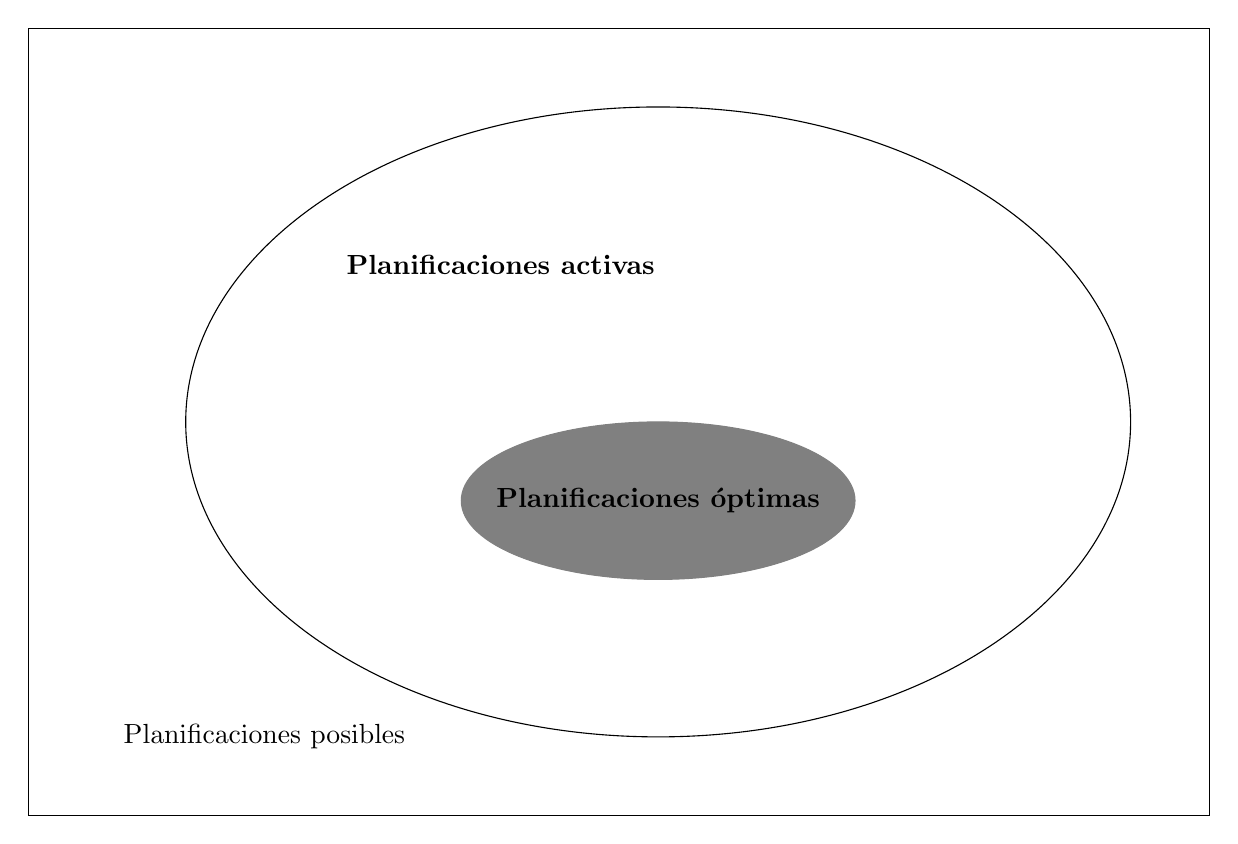
\begin{tikzpicture}
\draw (0,0) rectangle (15,10);  
\node [at={(3,1)}] {Planificaciones posibles};
\draw (8,5) ellipse[x radius = 6, 
y radius = 4];
    \node [at={(6,7)}] {\textbf{Planificaciones activas}};
    \draw[fill,color=gray]  (8,4) ellipse [x radius =2.5, 
y radius = 1];
    \node [at = {(8,4)}] {\textbf{Planificaciones \'optimas}};
\end{tikzpicture}

\end{document}
